\chapter{Двойные, тройные и n-кратные интегралы}\label{chap:multiple-integrals}\markright{Глава 44}

\section{От длины к площади и объёму}
\begin{definition}\term{Кратный интеграл Римана} (\emph{multiple Riemann integral}) по прямоугольному параллелепипеду \(B=\prod_{j=1}^n[a_j;b_j]\) определяется пределом сумм
\[
\sum_Q f(\xi_Q)\operatorname{vol}_n(Q)
\quad\text{при измельчении сетки},\qquad \xi_Q\in Q.
\]
Здесь \(Q\) — маленькие прямоугольные ячейки, \(\operatorname{vol}_n(Q)\) — произведение длин их сторон. Предел должен быть одним и тем же для любого выбора точек и сеток с наибольшим диаметром ячейки, стремящимся к нулю. Для \(n=2\) пишут \(\iint_Df\,dA\), для \(n=3\) — \(\iiint_Vf\,dV\), в общем случае — \(\int_Df(x)\,dx_1\cdots dx_n\).\end{definition}
\par\addvspace{5pt}\begin{lrbox}{\CatFlowBox}\begin{minipage}[t]{\linewidth}
\setlength{\parskip}{5pt}\setlength{\columnsep}{4.5mm}\setlength{\intextsep}{0pt}
\begin{wrapfigure}[9]{r}{54mm}
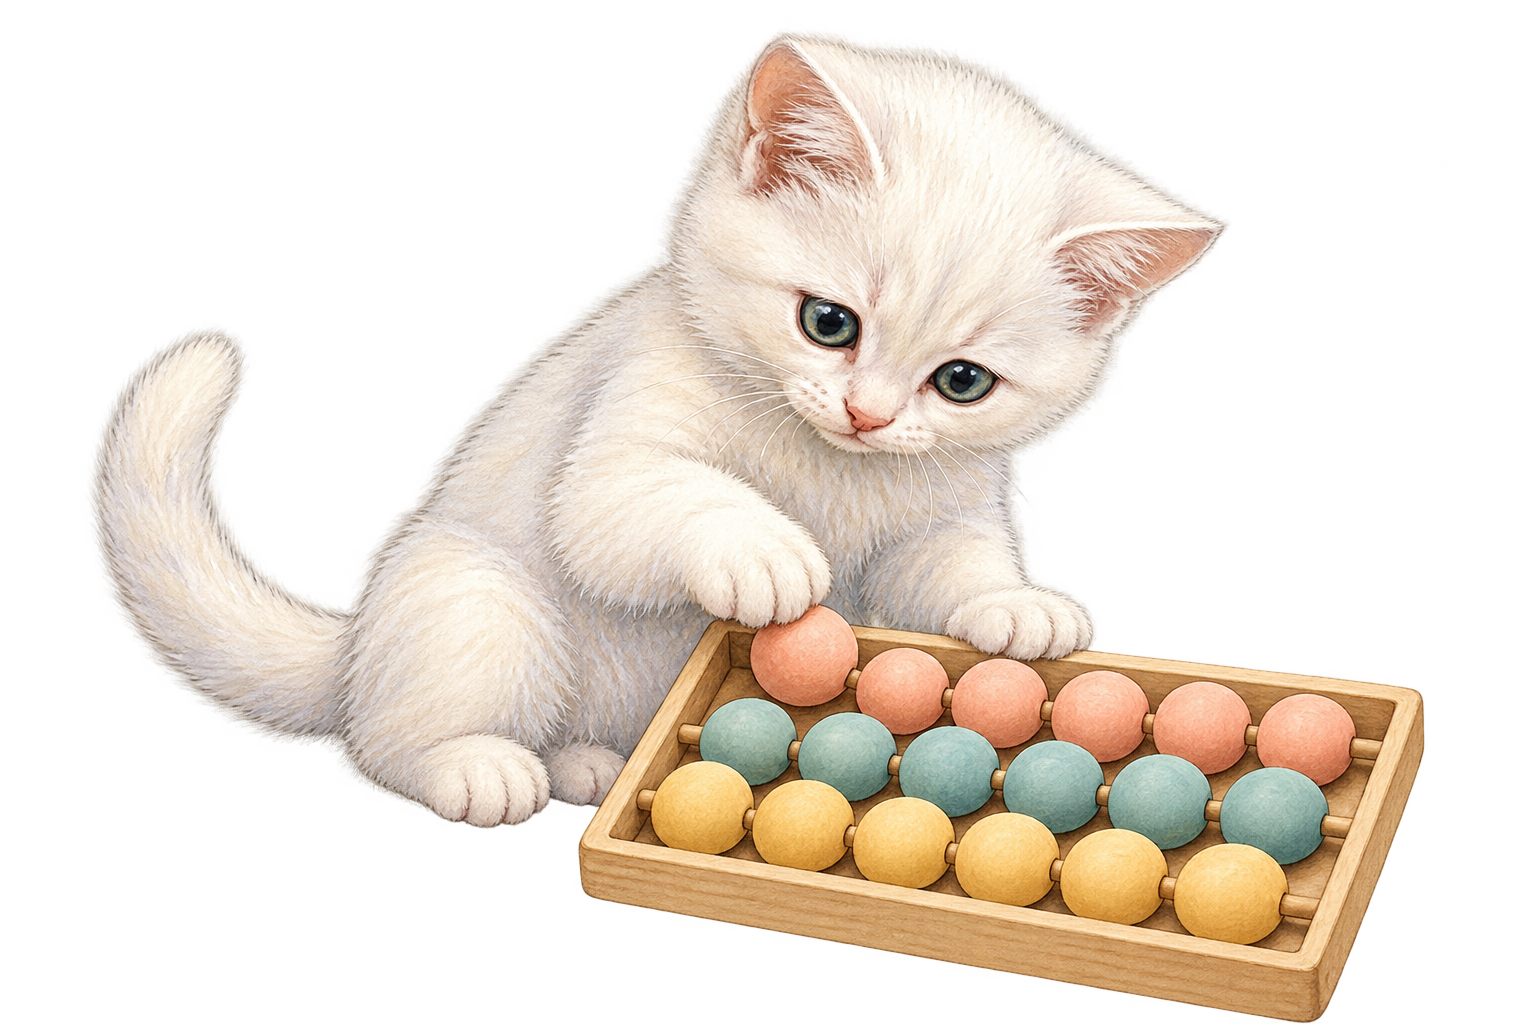
\includegraphics[width=54mm,height=58mm,keepaspectratio]{images/unique/art-154.png}
\label{catflow:154}
\end{wrapfigure}
Кратность интеграла задаёт число независимых координат области, а не степень подынтегральной функции. Двойной интеграл от \(1\) считает площадь плоской области, тройной — объём пространственного тела. Если подынтегральная функция является плотностью, результатом становится масса. Например, поверхностная плотность в килограммах на квадратный метр после умножения на площадь ячейки даёт килограммы.
\par\WFclear\end{minipage}\end{lrbox}%
\ifdim\dimexpr\ht\CatFlowBox+\dp\CatFlowBox\relax<64mm\dp\CatFlowBox=\dimexpr64mm-\ht\CatFlowBox\relax\fi%
\noindent\usebox{\CatFlowBox}\par\addvspace{5pt}
\begin{theorem}[Непрерывность и теорема Фубини на прямоугольнике; Fubini's theorem]
Непрерывная функция на замкнутом ограниченном прямоугольном параллелепипеде интегрируема. Её кратный интеграл равен повторному одномерному интегралу в любом порядке. В частности,
\[
\iint_{[a;b]\times[c;d]}f(x,y)\,dA
=\int_a^b\left(\int_c^d f(x,y)\,dy\right)dx.
\]
\end{theorem}
\begin{proof}Из любой последовательности точек параллелепипеда можно последовательно выделить сходящиеся подпоследовательности по каждой из конечного числа координат; предел остаётся в нём. Тем же противоречием, что в теореме Кантора на отрезке, получаем ограниченность и равномерную непрерывность \(f\). Поэтому колебания на всех ячейках мелкой сетки одновременно малы: разность верхней и нижней сумм не больше общего объёма, умноженного на наибольшее колебание. Это доказывает существование интеграла.

Для двух переменных \(g(x)=\int_c^d f(x,y)\,dy\) непрерывна, поскольку \(|g(x)-g(x')|\le(d-c)\max_y|f(x,y)-f(x',y)|\). На фиксированной мелкой сетке по \(x\) сумма \(\sum_i g(\xi_i)\Delta x_i\) отличается сколь угодно мало от двойной суммы Римана, если достаточно измельчить сетку по \(y\). Оценка равномерна по конечному числу \(\xi_i\). Устремляя мелкости к нулю, получаем формулу. Перестановка переменных даёт другой порядок. Индукция по числу координат доказывает общий случай.\end{proof}
\begin{definition}\term{Жорданова измеримость} (\emph{Jordan measurability}) ограниченной области означает, что её границу можно покрыть конечным числом прямоугольных ячеек со сколь угодно малым суммарным \(n\)-мерным объёмом. Для такой области интеграл задают продолжением ограниченной функции нулём на окружающий прямоугольник, если продолжение интегрируемо. У треугольников, кругов, многогранников и шаров граница обладает нужным свойством.\end{definition}
Для непрерывной функции на замкнутой ограниченной жорданово измеримой области нулевое продолжение интегрируемо. Объяснение критерия: ячейки у границы дают сколь угодно малый вклад за счёт ограниченности, а вдали от границы работают равномерная непрерывность и обычные суммы Римана.
\section{Двойные интегралы и переменные границы}
\begin{theorem}[Область между графиками]
Если \(g_1,g_2\) непрерывны, \(g_1\le g_2\) на \([a;b]\), а \(f\) непрерывна на
\[
D=\{(x,y):a\le x\le b,\ g_1(x)\le y\le g_2(x)\},
\]
то \(\displaystyle\iint_D f\,dA=\int_a^b\int_{g_1(x)}^{g_2(x)}f(x,y)\,dy\,dx\).
\end{theorem}
\begin{proof}Разобьём окружающий прямоугольник сеткой и продолжим \(f\) нулём. Ячейки, не пересекающие границы графиков, входят в область целиком либо не входят. Конечные суммы по внутренним ячейкам группируются сначала по столбцам. Ячейки, встречающие графики непрерывных \(g_i\), имеют сколь угодно малую суммарную площадь при измельчении: колебания \(g_i\) на узких полосах равномерно малы. Их вклад ограничен максимумом \(|f|\), умноженным на эту площадь. Предел сгруппированных сумм даёт указанную формулу.\end{proof}
\par\addvspace{5pt}\begin{lrbox}{\CatFlowBox}\begin{minipage}[t]{\linewidth}
\setlength{\parskip}{5pt}\setlength{\columnsep}{4.5mm}\setlength{\intextsep}{0pt}
\begin{wrapfigure}[11]{l}{54mm}

\includegraphics[width=54mm,height=58mm,keepaspectratio]{images/unique/art-155.png}
\label{catflow:155}
\end{wrapfigure}
Прежде чем менять порядок интегрирования, полезно нарисовать область и описать её неравенствами. Запись \(0\le y\le x\le1\) задаёт тот же треугольник, что \(0\le y\le1,\ y\le x\le1\). Поменять местами одни символы \(dx,dy\), сохранив старые зависимые пределы, нельзя: внутренние границы должны зависеть только от внешних переменных.
\par\WFclear\end{minipage}\end{lrbox}%
\ifdim\dimexpr\ht\CatFlowBox+\dp\CatFlowBox\relax<64mm\dp\CatFlowBox=\dimexpr64mm-\ht\CatFlowBox\relax\fi%
\noindent\usebox{\CatFlowBox}\par\addvspace{5pt}
Например,
\[
\iint_{\{0\le y\le x\le1\}}(x+y)\,dA
=\int_0^1\int_0^x(x+y)\,dy\,dx
=\int_0^1\frac32x^2\,dx=\frac12.
\]
\begin{definition}\term{Центр масс плоской пластинки} (\emph{center of mass}) с неотрицательной плотностью \(\rho\) и массой \(M=\iint_D\rho\,dA>0\) имеет координаты \(\bar x=\frac1M\iint_Dx\rho\,dA\), \(\bar y=\frac1M\iint_Dy\rho\,dA\).\end{definition}
\section{Тройные и \(n\)-кратные интегралы}
Для тела \(V=\{(x,y,z):(x,y)\in D,\ h_1(x,y)\le z\le h_2(x,y)\}\) с компактной жорданово измеримой \(D\), непрерывными на \(D\) границами \(h_1\le h_2\) и непрерывной на \(V\) функцией \(f\) соответствующий повторный интеграл имеет вид
\[
\iiint_V f\,dV=\iint_D\left(\int_{h_1(x,y)}^{h_2(x,y)}f(x,y,z)\,dz\right)dA.
\]
Обоснование такое же, как для области между графиками: приграничные ячейки дают исчезающий вклад, внутренние группируются в столбики.

При \(n\) переменных прямоугольник \(\prod_{j=1}^n[0;a_j]\), \(a_j>0\), имеет объём \(\prod_j a_j\). Для непрерывных \(g_j\) теорема Фубини даёт
\[
\int_{\prod_j[a_j;b_j]}\prod_{j=1}^ng_j(x_j)\,dx_1\cdots dx_n
=\prod_{j=1}^n\int_{a_j}^{b_j}g_j(t)\,dt.
\]
\subsection{Вывод формул объёма сечениями}\label{sec:solid-volume-integral}
\par\addvspace{5pt}\begin{lrbox}{\CatFlowBox}\begin{minipage}[t]{\linewidth}
\setlength{\parskip}{5pt}\setlength{\columnsep}{4.5mm}\setlength{\intextsep}{0pt}
\begin{wrapfigure}[11]{l}{54mm}

\includegraphics[width=54mm,height=58mm,keepaspectratio]{images/unique/art-157.png}
\label{catflow:157}
\end{wrapfigure}
\textit{Доказательство.} Объём тела равен \(\int A(z)\,dz\), где \(A(z)\) — площадь горизонтального сечения: это Фубини для интеграла от \(1\). У призмы и цилиндра \(A(z)=B\), поэтому \(V=Bh\). У пирамиды и конуса \(A(z)=B(1-\frac zh)^2\), \(0\le z\le h\), по подобию сечений. Отсюда \(V=B\int_0^h(1-\frac zh)^2dz=\frac13Bh\). У шара \(A(z)=\pi(R^2-z^2)\), \(-R\le z\le R\), поэтому \(V=\pi[R^2z-\frac{z^3}3]_{-R}^{R}=\frac43\pi R^3\).\hfill\(\blacksquare\)
\par\WFclear\end{minipage}\end{lrbox}%
\ifdim\dimexpr\ht\CatFlowBox+\dp\CatFlowBox\relax<64mm\dp\CatFlowBox=\dimexpr64mm-\ht\CatFlowBox\relax\fi%
\noindent\usebox{\CatFlowBox}\par\addvspace{5pt}

\section{Замена переменных и модуль якобиана}
\begin{theorem}[Многомерная замена переменных; change of variables]\label{thm:change-variables}
Пусть \(T\) — взаимно однозначное \(C^1\)-отображение открытой области в \(\mathbb R^n\) на другую открытую область, обратное также класса \(C^1\), а \(\det DT\ne0\). Для компактной жорданово измеримой области \(G\) внутри области определения и непрерывной \(f\) на \(T(G)\)
\[
\int_{T(G)}f(x)\,dx
=\int_G f(T(u))\,|\det DT(u)|\,du.
\]
\end{theorem}
Общая теорема приведена без полного доказательства. Её геометрическая основа — замена малого блока линейным приближением \(DT\): его объём умножается на \(|\det DT|\). Модуль необходим, потому что геометрическая площадь и объём не становятся отрицательными при отражении. Для полярных и сферических координат формулу применяют в области без вырожденных точек и шва; исключённые границы имеют нулевую площадь или объём и интеграл не меняют.

\begin{definition}\term{Полярные координаты} (\emph{polar coordinates}) на плоскости: \(x=r\cos\theta,\ y=r\sin\theta\), \(r\ge0\). Элемент площади \(dA=r\,dr\,d\theta\).\end{definition}
\begin{definition}\term{Цилиндрические координаты} (\emph{cylindrical coordinates}): \(x=r\cos\theta,\ y=r\sin\theta,\ z=z\). Элемент объёма \(dV=r\,dr\,d\theta\,dz\).\end{definition}
\begin{definition}\term{Сферические координаты} (\emph{spherical coordinates}) в выбранном соглашении:
\[
x=\rho\sin\varphi\cos\theta,\quad
y=\rho\sin\varphi\sin\theta,\quad z=\rho\cos\varphi.
\]
Здесь \(\rho\ge0,\ 0\le\varphi\le\pi,\ 0\le\theta<2\pi\); \(dV=\rho^2\sin\varphi\,d\rho\,d\varphi\,d\theta\). Полярный угол \(\varphi\) отсчитывается от положительной оси \(z\).
\end{definition}
\par\addvspace{5pt}\begin{lrbox}{\CatFlowBox}\begin{minipage}[t]{\linewidth}
\setlength{\parskip}{5pt}\setlength{\columnsep}{4.5mm}\setlength{\intextsep}{0pt}
\begin{wrapfigure}[10]{r}{54mm}
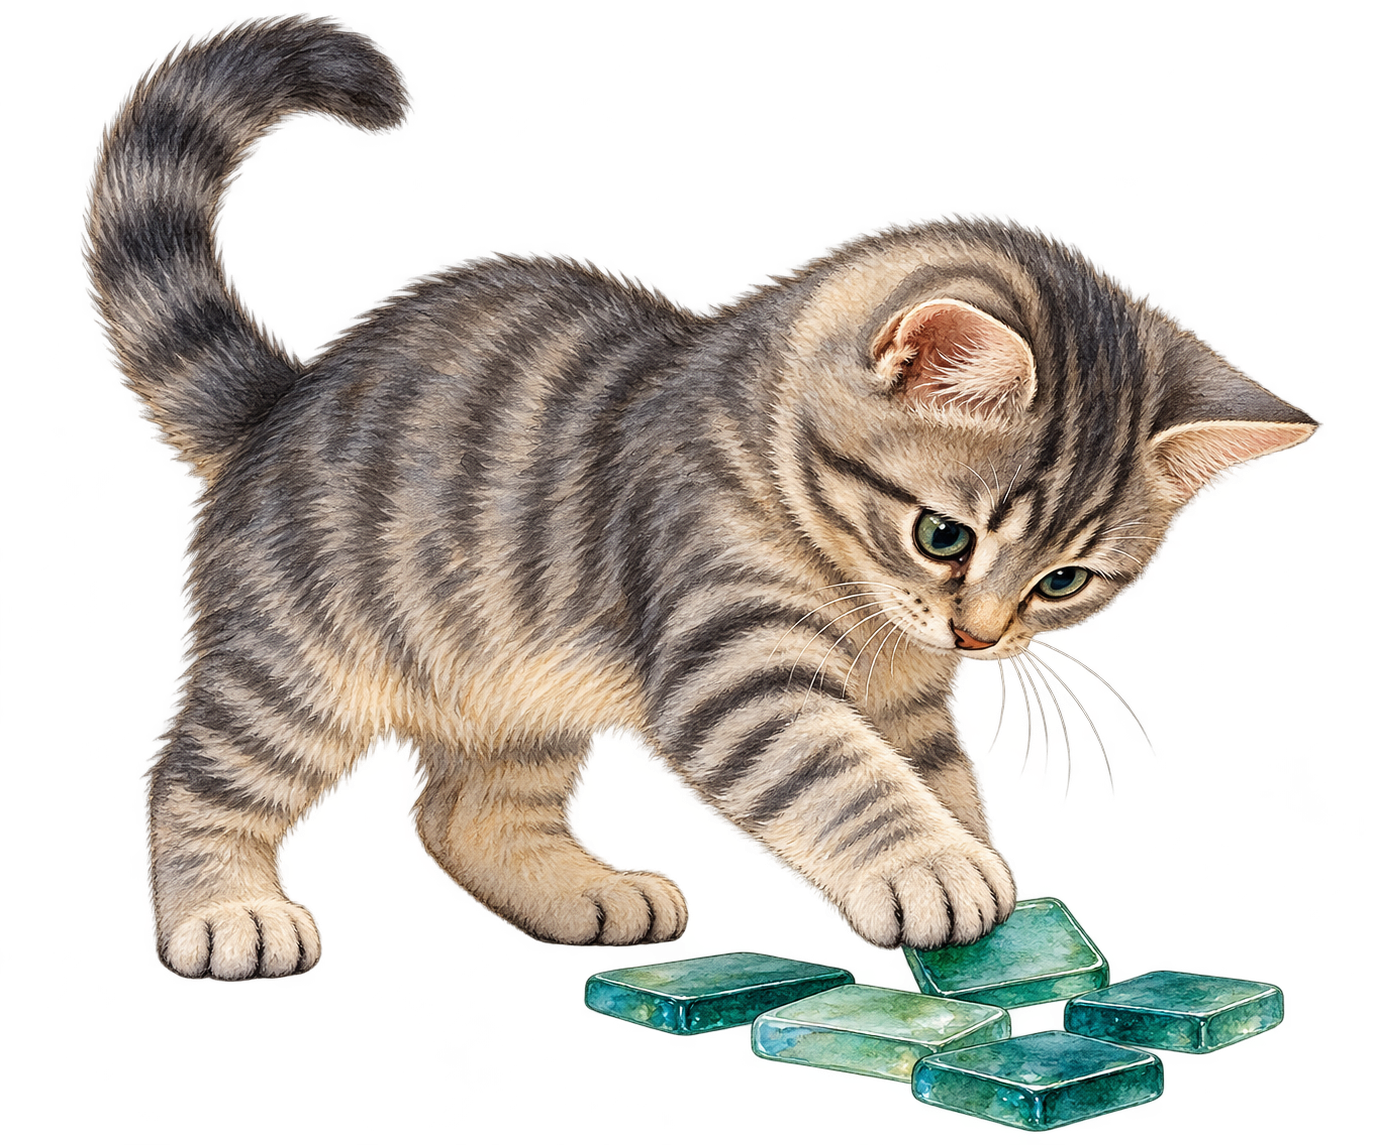
\includegraphics[width=54mm,height=58mm,keepaspectratio]{images/unique/art-156.png}
\label{catflow:156}
\end{wrapfigure}
Удобные координаты упрощают область, но меняют элемент площади или объёма. В полярных координатах маленький сектор имеет радиальную сторону \(dr\) и поперечную длину примерно \(r\,d\theta\); поэтому появляется множитель \(r\). Без него интеграл по кругу дал бы величину неправильной размерности. В сферических координатах две угловые стороны дают множитель \(\rho^2\sin\varphi\).
\par\WFclear\end{minipage}\end{lrbox}%
\ifdim\dimexpr\ht\CatFlowBox+\dp\CatFlowBox\relax<64mm\dp\CatFlowBox=\dimexpr64mm-\ht\CatFlowBox\relax\fi%
\noindent\usebox{\CatFlowBox}\par\addvspace{5pt}
Например, для круга радиуса \(R\)
\[
\iint_{x^2+y^2\le R^2}(x^2+y^2)\,dA
=\int_0^{2\pi}\int_0^R r^3\,dr\,d\theta=\frac{\pi R^4}2.
\]

\par\noindent\begin{minipage}{\linewidth}\section*{Графики}
\begin{center}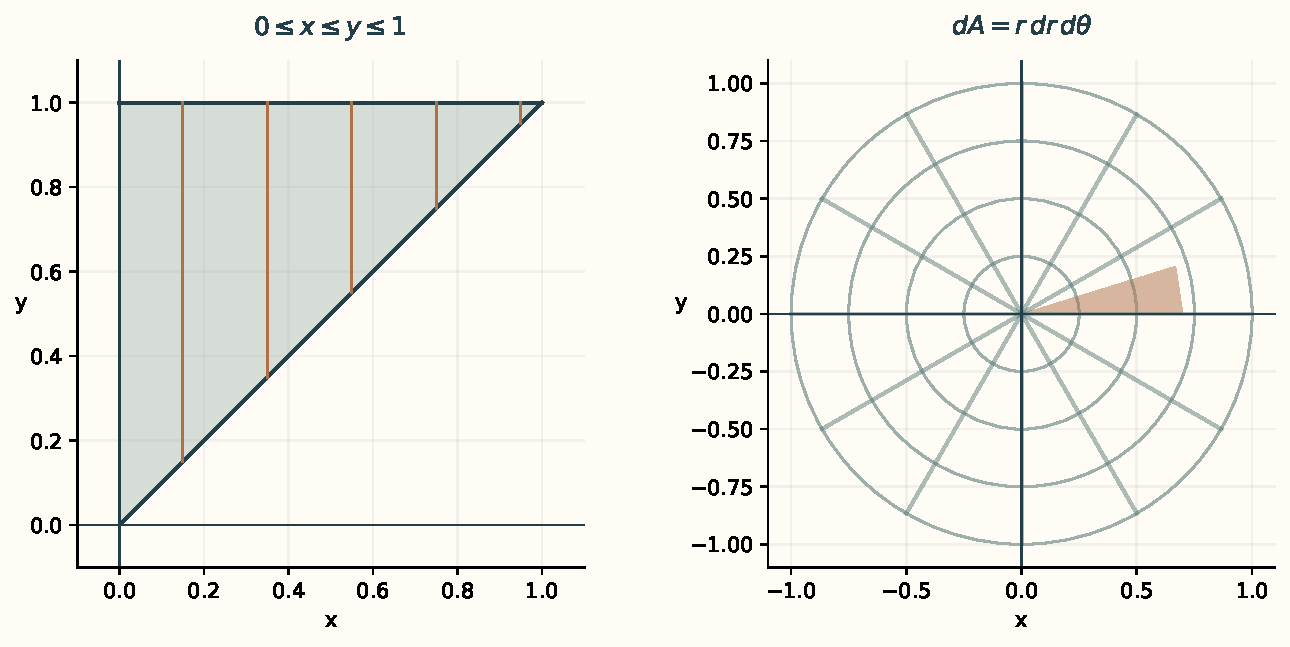
\includegraphics[width=\textwidth,height=.79\textheight,keepaspectratio]{images/atlas-multiple-integrals.pdf}\par\small Область интегрирования и замена координат\end{center}\end{minipage}\par
\Needspace{7\baselineskip}\section*{Задачи}
\begingroup\setlength{\parskip}{2pt}
\noindent\begin{minipage}[t]{\linewidth}\textbf{44.1.} Вычисли \(\iint_D1\,dA\), где \(D=[0;2]\times[0;3]\).\par\end{minipage}\par
\noindent\begin{minipage}[t]{\linewidth}\textbf{44.2.} Вычисли \(\iint_{[0;1]^2}(x+y)\,dA\).\par\end{minipage}\par
\noindent\begin{minipage}[t]{\linewidth}\textbf{44.3.} Вычисли \(\iint_{[0;2]\times[0;1]}xy\,dA\).\par\end{minipage}\par
\noindent\begin{minipage}[t]{\linewidth}\textbf{44.4.} Вычисли \(\iint_{[0;1]^2}(x^2+y^2)\,dA\).\par\end{minipage}\par
\noindent\begin{minipage}[t]{\linewidth}\textbf{44.5.} Для треугольника \(0\le y\le x\le1\) найди площадь и интеграл от \(x+y\).\par\end{minipage}\par
\par\addvspace{5pt}\begin{lrbox}{\CatFlowBox}\begin{minipage}[t]{\linewidth}
\setlength{\parskip}{5pt}\setlength{\columnsep}{4.5mm}\setlength{\intextsep}{0pt}
\begin{wrapfigure}[11]{r}{54mm}

\includegraphics[width=54mm,height=58mm,keepaspectratio]{images/unique/art-158.png}
\label{catflow:158}
\end{wrapfigure}
\textbf{44.6.} Вычисли \(\iint_Dx\,dA\) по треугольнику \(x\ge0,y\ge0,x+y\le1\).\par

\textbf{44.7.} Перепиши \(\int_0^1\int_x^1 f(x,y)\,dy\,dx\) в обратном порядке для непрерывной \(f\).\par

\textbf{44.8.} Найди площадь круга радиуса \(2\) через полярный двойной интеграл.\par

\textbf{44.9.} Вычисли \(\iint_{x^2+y^2\le4}(x^2+y^2)\,dA\).\par
\par\WFclear\end{minipage}\end{lrbox}%
\ifdim\dimexpr\ht\CatFlowBox+\dp\CatFlowBox\relax<64mm\dp\CatFlowBox=\dimexpr64mm-\ht\CatFlowBox\relax\fi%
\noindent\usebox{\CatFlowBox}\par\addvspace{5pt}

\noindent\begin{minipage}[t]{\linewidth}\textbf{44.10.} На кольце \(1\le\sqrt{x^2+y^2}\le2\) вычисли интеграл от \(\dfrac1{\sqrt{x^2+y^2}}\).\par\end{minipage}\par
\noindent\begin{minipage}[t]{\linewidth}\textbf{44.11.} У квадратной пластинки \(D=[0;1]^2\) плотность \(\rho=x+y\). Найди массу и центр масс.\par\end{minipage}\par
\noindent\begin{minipage}[t]{\linewidth}\textbf{44.12.} Вычисли \(\iiint_{[0;1]\times[0;2]\times[0;3]}xyz\,dV\).\par\end{minipage}\par
\noindent\begin{minipage}[t]{\linewidth}\textbf{44.13.} Найди объём тетраэдра \(x,y,z\ge0,\ x+y+z\le1\) тройным интегралом.\par\end{minipage}\par
\noindent\begin{minipage}[t]{\linewidth}\textbf{44.14.} Найди объём единичного шара в сферических координатах.\par\end{minipage}\par
\noindent\begin{minipage}[t]{\linewidth}\textbf{44.15.} Найди объём цилиндра радиуса \(2\) и высоты \(3\) в цилиндрических координатах.\par\end{minipage}\par
\noindent\begin{minipage}[t]{\linewidth}\textbf{44.16.} Вычисли интеграл от \(z\) по шару \(x^2+y^2+z^2\le R^2\).\par\end{minipage}\par
\noindent\begin{minipage}[t]{\linewidth}\textbf{44.17.} Вычисли \(n\)-кратный интеграл \(\int_{[0;1]^n}x_1\cdots x_n\,dx_1\cdots dx_n\).\par\end{minipage}\par
\noindent\begin{minipage}[t]{\linewidth}\textbf{44.18.} Вычисли \(n\)-кратный интеграл от \(1\) по \(\prod_{j=1}^n[0;a_j]\), где \(a_j>0\).\par\end{minipage}\par
\noindent\begin{minipage}[t]{\linewidth}\textbf{44.19.} Преобразование \(x=-u,y=v\) отражает единичный квадрат. Найди якобиан и площадь образа. Объясни, зачем в замене переменных модуль.\par\end{minipage}\par
\noindent\begin{minipage}[t]{\linewidth}\textbf{44.20.} При \(x=2u,y=3v\), \(0\le u,v\le1\), вычисли интеграл от \(x+y\) по образу квадрата.\par\end{minipage}\par
\noindent\begin{minipage}[t]{\linewidth}\textbf{44.21.}\starmark{} Вычисли определитель сферического преобразования по \((\rho,\varphi,\theta)\) и проверь элемент объёма.\par\end{minipage}\par
\noindent\begin{minipage}[t]{\linewidth}\textbf{44.22.}\starmark{} Вычисли \(\iiint_{x^2+y^2+z^2\le R^2}(x^2+y^2+z^2)\,dV\).\par\end{minipage}\par
\noindent\begin{minipage}[t]{\linewidth}\textbf{44.23.}\starmark{} Пусть \(I_R=\int_{-R}^Re^{-x^2}\,dx\). Сравни интеграл от \(e^{-x^2-y^2}\) по квадрату \([-R;R]^2\) с интегралами по кругам радиусов \(R,\sqrt2R\). Докажи \(\lim_{R\to\infty}I_R=\sqrt\pi\).\par\end{minipage}\par
\noindent\begin{minipage}[t]{\linewidth}\textbf{44.24.}\starmark{} Докажи формулу произведения интегралов для \(\prod_{j=1}^ng_j(x_j)\) на прямоугольнике, предполагая непрерывность всех \(g_j\).\par\end{minipage}\par
\endgroup
